%% LyX 2.2.0 created this file.  For more info, see http://www.lyx.org/.
%% Do not edit unless you really know what you are doing.
\documentclass[12pt,english]{kuthesis}
\usepackage{mathptmx}
\usepackage{MnSymbol}
\renewcommand{\sfdefault}{lmss}
\renewcommand{\ttdefault}{lmtt}
\usepackage[T1]{fontenc}
\usepackage[utf8]{inputenc}
\usepackage{geometry}
\geometry{verbose,tmargin=1in,bmargin=1in,lmargin=1in,rmargin=1in}
\setcounter{secnumdepth}{3}
\setcounter{tocdepth}{3}
\usepackage{xcolor}
\usepackage{babel}
\usepackage{url}
\usepackage{graphicx}
\usepackage{setspace}
\usepackage{esint}
\usepackage[authoryear]{natbib}
\usepackage{bussproofs}
\usepackage{semantic}

\doublespacing
\usepackage[unicode=true,
 bookmarks=true,bookmarksnumbered=false,bookmarksopen=false,
 breaklinks=true,pdfborder={0 0 0},pdfborderstyle={},backref=false,colorlinks=true]
 {hyperref}
\hypersetup{pdftitle={University of Kansas Thesis Template},
 pdfauthor={Apoorv Ingle},
 pdfsubject={A Thesis},
 urlcolor={black},citecolor={black},allcolors={black}}

\makeatletter

%%%%%%%%%%%%%%%%%%%%%%%%%%%%%% LyX specific LaTeX commands.
\providecommand{\LyX}{\texorpdfstring%
  {L\kern-.1667em\lower.25em\hbox{Y}\kern-.125emX\@}
  {LyX}}
%% Because html converters don't know tabularnewline
\providecommand{\tabularnewline}{\\}

%%%%%%%%%%%%%%%%%%%%%%%%%%%%%% User specified LaTeX commands.


%used to align decimals in tables according to APA style
\usepackage{dcolumn}
\usepackage{booktabs}

% Set the title and author info
\title{Resource Aware Functional Language}
\author{Apoorv Ingle}


\dept{Electrical Engineering and Computer Science}
\degreetitle{Master of Science}
\papertype{Thesis} %or Thesis (Whatever you put will appear on p.2)
%% It is vital to have 7 entries, even if some are empty for committee and role
%% I mean, it is vital to leave the empty place holders
\committee{Dr. J. Garrett Morris}{Dr. Perry Alexandar}{Dr. Andy Gill}{Dr. Prasad Kulkarni}{}{}{}
\role{Chairperson}{Dr. J. Garrett Morris}{}{}{}{}{}
%AT Most 7 members allowed, last here is blank on purpose to demonstrate
%flexibility

%% The following is OPTIONAL. Remove all 3 of the next 3 lines
%% to leave dates blank. If dates are included, then both dates
%% must be included.
\@printd@testrue
\datedefended{July 21, 2018}
\dateapproved{July 21, 2018}

%% These settings are now in the kuthesis.cls file, but users are free
% to customize. listings has great documentation online
%% When listings are used, break lines
%\lstset{
 %    breaklines=true,  % sets automatic line breaking
 %    breakindent=2em,
 %    breakatwhitespace=true,  % sets if automatic breaks should
 %   breakautoindent=true
%}

\@ifundefined{showcaptionsetup}{}{%
 \PassOptionsToPackage{caption=false}{subfig}}
\usepackage{subfig}
\makeatother

\usepackage{listings}
\renewcommand{\lstlistingname}{\inputencoding{latin9}Listing}

\begin{document}
\begin{romanpages}

\maketitle
\begin{abstract}

  What am i doing here?
  Make Quill work. Write programs in them and check and see
  how painful it is.

  Quill is a purely functional language that uses
  qualified types to keep track of resources.
  We introduce a new type class to express unrestrictedness
  of a type, define the degree of unrestrictedness of classes
  and a concept of sharing or separation of closures for functions

% How to use these files.

% \textbf{Step 1. Study the features in this document.} Please read
% through this Abstract. It is intended to be readable, pleasant, welcoming
% and helpful. The PDF you are reading was created by compiling thesis-ku.tex.
% After you finish inspecting this document, then look at the LaTeX
% document from which it came. 

% \textbf{Step 2. Inspect the LaTeX source code that is provided in
% the same package as the PDF document.}

% There are some special features that will become apparent once you
% look at the LaTeX source code. The thesis-ku document is the ``master''
% document. The separate chapters are in separate folders. It is possible
% to work on one chapter at a time, and compile just that chapter, or
% it is possible to compile the whole thing by compiling the master
% document.

% In thesis-ku, we have included as many bells and whistles as possible
% so that users can see how the different features can be put to use.
% We have a BibTeX bibliography, graphs, equations, cross references,
% table of contents, and all of the other interesting features.

% The most recently inserted feature is support for hyperlinks in the
% PDF output. We checked with the KU Graduate Dean's office and they
% said there is no policy prohibiting the use of hyperlinks, but there
% is also no guarantee from the dissertation hosting institution that
% they will either work or not cause problems down the line. We believe
% there is not too much danger here, this feature is easy to turn off
% if need be. Also, it is not entirely clear what color the links must
% be inside the document, so we take a conservative step here of making
% the links black, so they appear as simple text. The default settings
% for the \texttt{hyperref} package, which we have altered, caused ugly
% pink links with gross looking boxes around them. Users can change
% the link color to blue. It is fairly easy to see how this can be done
% in the document preamble. Look for something like this ``\texttt{urlcolor=\{black\},citecolor=\{black\},allcolors=\{black\}''}
% and think of Henry Ford's famous comment, ``You can have a car in
% any color you like, as long as its black.'' 

% \textbf{Step 3. Try to compile the thesis-ku document!} Before you
% try to edit this and enhance it (and put your name on it), please
% \textbf{STOP}! Recompile this document exactly as it is. This will
% force you to test your LaTeX setup. Unzip the collection, consider
% installing the class file as described below, then try to compile
% \texttt{thesis-ku}. That zipped collection has everything in the right
% places, don't re-arrange directories yet. Until you reproduce the
% PDF you are reading now, you are not ready to start making changes.
% People often come forward with questions and our first question for
% them is ``did you compile (without error) \texttt{thesis-ku.tex}?''
% Until we hear those people say ``yes'', we are generally unable
% to help with their revised documents. That's the only way we will
% know if your \LaTeX{} setup is ready to go. 

% \emph{If you have used \LaTeX{}}, you will find this more or less
% self explanatory. There's a \LaTeX{} file ``\texttt{thesis-ku.tex}''.
% It is a ``master'' document, it links together the content of several
% files. Compile that with \texttt{\textbf{pdflatex}}. The class file
% that makes this go, ``\texttt{kuthesis.cls}'', is saved in the current
% working directory. It is not necessary to install it into your broader
% \LaTeX{} distribution, but you can if you like. One reason to install
% kuthesis.cls in your larger setup is to silence warnings from editors
% that don't remember to look in your current directory. If you install
% \texttt{kuthesis.cls} in your system, you don't need to keep a copy
% of it with your dissertation. That may be convenient.

% \emph{If you have never used \LaTeX{}}, we will tell you how to compile
% this document. But, before you try, can we give you a warning: \emph{please
% don't make writing your dissertation your first \LaTeX{} project}.
% Start with some simpler example documents. Write some letters to your
% loved ones, experiment a little bit. In the KU Center for Research
% Methods and Data Analysis, there are occasional workshops for people
% who want to get started with \LaTeX{}. There are many ``how to get
% started with \LaTeX{}'' websites. Ours is \url{http://crmda.ku.edu/latex}.

% If you have never used LaTeX before, a good way to start is with the
% editor named LyX. Instead of editing the ``raw'' LaTeX file \texttt{thesis-ku.tex},
% use LyX to edit \texttt{thesis-ku.lyx}. There is a separate section
% below about using LyX.

% \textbf{Step 4. Customize This and Write a Dissertation.}
% This PDF document is produced from a source document. If you are using
% a \LaTeX{} editor like TexShop, Tex Works, or \TeX{} Studio, the
% source document you need to edit and compile is ``\texttt{thesis-ku.tex}.''
% If you plan to use \LyX{}, the place to start is by opening ``\texttt{thesis-ku.lyx}''
% in \LyX{}'s editor. This document was prepared with version 2.1 and,
% if you are using an older version, you should update.

% The first user customization is to insert your name and the names
% of some committee members. The document has a top section called a
% ``preamble.'' (If using \LyX{}, click the Document menu, then Settings,
% and look down). In the preamble, you will find the following block:

% \inputencoding{latin9}\begin{lstlisting}[tabsize=4]
% % Set the title and author info
% \title{Resource Aware purely functional language}
% \author{Apoorv Inge}

% \dept{Electrical Engineering and Computer Science}
% \degreetitle{Master of Science}
% \papertype{Thesis} %or Thesis
%% It is vital to have 7 entries, so leave the empty place holders {} even 
%% if some of the committee and role lines are to remain empty
% \committee{MEMBER 1}{MEMBER 2}{MEMBER 3}{MEMBER 4}{The One with an Extra Long Name}{The Fifth Beatle}{}
% \role{Chairperson}{Occasional Visitor}{}{The One Who Never Answers Email}{}{}{}
% \end{lstlisting}
% \inputencoding{utf8}
% Here you see the most important template updates for October, 2015.
% We have newly enhanced \texttt{\textbackslash{}committee} and \texttt{\textbackslash{}role}
% environments. Now, we allow users to specify up to 7 committee members
% and each one can have a different role. Why provide all of this luxury?
% There were unexpected requests from students. The original KU Thesis
% template had only ``Chair'' for the first member. Users asked for
% a secondary title ``Co-Chair'' for member 2. Then they wanted to
% change the title of the first member to ``Lead Chair''. Then they
% wanted to add a the third Co-Chair, and so forth. 

% Now we accommodate those requests by leaving blank spots for up to
% seven committee members and seven roles. It is vital for you to leave
% the blank place holders \{\} if you don't want to list additional
% members or roles. This example document shows some funny titles, we
% do that only to prove it is possible. Generally, there is only a Chair,
% possibly a Co-Chair. This example has more roles in this example for
% fun. Or to make fun of a professor. You can change them to \{\}, of
% course, if you don't want a named role.

% The other thing to change is the date section. Lower in the preamble,
% you should see a place to insert some dates. Originally, we told students
% ``just write those dates in by hand, like we did back in the olden
% days.'' But they kept saying they wanted them type set, so here they
% are. If a date is currently unknown, just leave a blank inside the
% brackets
% \inputencoding{latin9}\begin{lstlisting}
% \datedefended{June 11, 2018}
% \dateapproved{June 11, 2018}
% \end{lstlisting}
% \inputencoding{utf8}
% After you make those changes in the preamble, compile the document.

% \textbf{How to Configure your LaTeX Distribution with kuthesis.cls}

% I wish we had packaged \texttt{kuthesis.cls} into an official LaTeX
% distribution package so that it could be easily installed by your
% distribution. We did not do that, however, and so it is up to you
% to place a copy of \texttt{kuthesis.cls} in the right spot\texttt{.}
% This is not truly necessary. Programs like pdflatex will find \texttt{kuthesis.cls}
% if you have it in the same directory as the document. I believe, with
% 97.5\% confidence, it will find \texttt{kuthesis.cls} if you keep
% it in the same directory as your document. If you want to use kuthesis.cls
% for several documents, it is necessary to install ``\texttt{kuthesis.cls}''
% into your \LaTeX{} file structure. That is generally an easy process,
% but it is different on every type of computer. The CRMDA staff has
% recently prepared a guide for this, entitled ``How Users can Install
% \LaTeX{} packages without Help from System Administrators'' (\url{https://crmda.ku.edu/guide-32-latex_config}).
% The gist of this is as follows:

% \begin{enumerate}
% \item Copy ``\texttt{kuthesis.cls}'' into a directory in your \LaTeX{}
% distribution. Usually (almost always), you will find a directory component
% that ends in ``tex/latex'' and you can put kuthesis.cls in there.
% The only puzzle is finding the right place, and that's why you should
% review our guide.{\small \par}
% \item Run ``texhash'' or to make the \LaTeX{} distribution take notice
% of your new file. On Mac and Linux systems, open a terminal and run
% ``\texttt{sudo texhash}'' to get this done as the administrator.{\small \par}
% \end{enumerate}
% \textbf{How to Get Started on this with \LyX{}}

% This document with \LyX{}! It will work. LyX is a pleasant-to-use
% editor, it can protect you from some of the details that ordinary
% \LaTeX{} will present. \LyX{} is free to use on all major computing
% platforms, including Linux, Macintosh, and Windows. \LyX{} can be
% downloaded at \url{http://www.lyx.org}. To make this work, LaTeX
% programs are also needed. 
% \begin{enumerate}
% \item Mac users: install the ``MacTeX'' package (\url{https://www.tug.org/mactex}). {\small \par}
% \item Linux users: install your distribution's version of TeXLive or install
% the TeXLive files from the TeXLive website (\url{https://www.tug.org/texlive})
% . {\small \par}
% \item Windows Users: The LyX website offers 2 choices, a LyX-only package
% and an ``installer bundle'' that includes LyX along with a small
% subset of the MikTeX LaTeX distribution. This installs just a small
% subset of MikTeX and pieces can be separately downloaded when needed.
% In Fall, 2016, we had some difficulties during a LaTeX workshop because
% the MikTeX package server was unavailable. As a result, we have been
% migrating away from MikTeX (and the LyX installer bundle) to use TeXLive
% for Windows (\url{https://www.tug.org/texlive}). That's a big 2GB
% package like MacTeX, after that we install the LyX program. If you
% choose the MikTeX setup instead, it will usually be fine, but users
% often complain that LyX seems to ``freeze'' when it downloads new
% MikTeX components.{\small \par}
% \end{enumerate}
%
% {\small \par}If you install a LaTeX distribution and LyX, then you can open the
% file ``thesis-ku.lyx''. At the very beginning, a couple of horrible
% warnings appear. These warnings look like this:

% \begin{tabular}{cc}
% 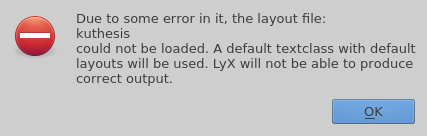
\includegraphics[width=2in]{images/lyx-nolayout} & 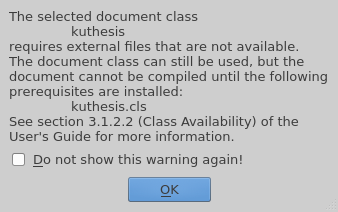
\includegraphics[width=2.5in]{images/lyx-noclsfile}\tabularnewline
% \end{tabular}

% We will explain how to eliminate these warnings, but you can ignore
% them for the moment. Just click ``OK'' 5 or 6 times. After that,
% you will find that the dissertation document can be compiled (even
% though there were horrible scary warnings). To compile the document,
% either click on the ``googly eyes'' icon in the toolbar or use the
% keyboard shortcut ``Ctl-R''. If your system has a PDF viewer installed
% and LyX can find it, all will be well. We are warned by Windows 10
% users that Microsoft has made the Web browser ``Edge'' the default
% PDF viewer and that does not work well with LyX. We recommend installing
% the PDF viewer Sumatra (\url{https://www.sumatrapdfreader.org/free-pdf-reader.html})
% and then using the Windows configuration to set Sumatra as the default
% PDF viewer.

% Why does \LyX{} work? When the user asks \LyX{} to preview the PDF
% output, a two step process happens behind the scenes. A file named
% ``\texttt{thesis-ku.tex}'' is created in a temporary directory,
% and then a program like \texttt{\textbf{pdflatex}} is asked to turn
% that into a PDF document. \LyX{} will then send the PDF output to
% a PDF viewer, such as Yapp, Evince or Acrobat.

% How to silence the LyX warnings.

% \noindent \textbf{1. Copy the LyX layout file ``}\texttt{\textbf{kuthesis.layout}}\textbf{''
% into the layout folder of the user configuration.}

% The only problem is finding the correct user configuration folder.

% {\small \par}\begin{description}
% \item [{On~Linux,}] copy \texttt{kuthesis.layout} into the user HOME folder,
% under ``\texttt{.lyx/layouts}''. {\small \par}
% \item [{On~Windows,}] there is a hidden AppData directory inside the user's
% home folder. How to find it? Run \LyX{}. A window should appear with
% a row of pull down menus at the top. Choose Tools/Preferences. Change
% something trivial, then close the menu. That will force \LyX{} to
% create a user folder. Then search inside your user directory for a
% key word such as ``lyxrc.defaults''. Probably, searching for ``{*}lyx{*}''
% will be sufficient. In MS Windows 7, I found ``C:\textbackslash{}Users\textbackslash{}pauljohn\textbackslash{}AppData\textbackslash{}Roaming\textbackslash{}lyx212\textbackslash{}layouts''.
% Caution: The AppData folder is hidden/concealed and, in order to find
% it in Windows Explorer, it is necessary to change the folder options
% to NOT hide protected files and folders. Windows 10 is very similar.{\small \par}
% \item [{On~Macintosh~OS~X,}] we recently followed same ``change a setting,
% then search'' procedure. The answer was ``/Users/pauljohn/Library/Application
% Support/\LyX{}-2.1/layouts''. Documentation for OS X El Capitan
% indicates that Apple has followed the Microsoft policy of hiding this
% folder, so the person who uses the Finder will have to change some
% preferences to show the directory.{\small \par}
% \end{description}
% \textbf{2. Copy the LaTeX class file ``}\texttt{\textbf{kuthesis.cls}}\textbf{''
% into the LaTeX distribution and then do the appropriate reconfiguration. }

% Again, if you have done this before, it is no big deal. If you have
% not done it before, it seems daunting. We described it in an earlier,
% under the heading \textbf{How to Configure your LaTeX Distribution
% with kuthesis.cls}. 

% \noindent \textbf{3. Let LyX find your changes.}

% \noindent In LyX, find the pull down menu item Tools -> Reconfigure. 

% After that, LyX should work and not warn you about files it thinks
% it does not have. Once again, it is not necessary to do these reconfigurations,
% but LyX will not warn about missing pieces anymore.

% We notice that LyX is not, by default, configured to do spell-checking
% as you type. This is a vestigial setting, a reflection of the days
% long ago when people knew how to spell. To turn on the spell checker,
% use the pull down menu \texttt{Tools} -> \texttt{Preferences} -> \texttt{Language
% Settings} -> \texttt{Spellchecker}. One must choose a program to serve
% as the ``Spellchecker engine'' and then click ``Spellcheck Continously''.
% The Spellchecker engine I use in Ubuntu Linux is called Enchant. I
% expect you will find one in your operating system, or can find one.
% If not, we may have to ask Mr. Google for help.

% \textbf{Other friendly advice.}

% \emph{Compile Early, Compile Often}

% The truly bad part of using \LaTeX{} is that the errors and warnings
% are, generally, not understandable. They are not understandable to
% me and I've been using \LaTeX{} for about 20 years. I mean, well,
% they are simply too abstract. Too complicated. If you insert an illegal
% character, such as an ``\_'' in a \LaTeX{} box, the document will
% fail with this unhelpful message

% \inputencoding{latin9}\begin{lstlisting}[breaklines=true,tabsize=2]
% Missing $ inserted.
% Missing $ inserted.
% Missing } inserted.
% Extra }, or forgotten \endgroup.
% ...
% I've inserted a begin-math/end-math symbol since I think you left one out. Proceed, with fingers crossed.
% \end{lstlisting}
% \inputencoding{utf8}
% \noindent At best, the message will point to the line you inserted
% to cause the problem, but often the \LaTeX{} system cannot guess
% where your mistake is, it can only say something is wrong. The best
% way to defend yourself: \textbf{\textit{Compile Early, Compile Often}}\textbf{.
% }Don't make a lot of changes without trying to compile. It is easy
% to insert a feature that breaks the document. Compile often so you
% know when things have gone wrong. 

% \emph{Use a Version Management System!}

% If this is an important project, please consider installing Git or
% some other version management program. It is difficult to avoid clutter
% if you have to rename your file every day. I see user directories
% full of files named, ``my\_diss.lyx'', ``my\_diss.2.lyx'', ``my\_diss\_final.lyx'',
% ``my\_diss\_rejected.lyx'' and so forth. It is very difficult to
% keep old and new versions straight unless you use a version manager.
% A version manager will handle that for you. You will just have one
% file ``my\_diss.lyx'' and you will have the ability to compare old
% and new snapshots. The CRMDA has a more-or-less comprehensive, yet
% easy to follow guide for Git, ``Git it Together''.

% I urge you to keep your \LaTeX{} document in Git so you can make
% frequent commits and it will be easy to step back in time. This is
% one reason why you should work on separate chapters, so if you break
% something, then you are more likely to find your mistakes.

% \emph{KU requires that fonts be compiled with the final result}

% The pdflatex compiler will insert fonts when it compiles the document.
% However, there is a ``gotcha''. If you create PDF documents separately,
% and you forget to embed the fonts with them, then the KU Graduate
% Dean's office is likely to reject your thesis. When a PDF is included
% within this document, pdflatex does not check to see if fonts are
% embedded in those PDFs. It assumes they are as you want them; fonts
% for those included files are not automatically inserted by pdflatex.
% When a graph, for example, is created in R and exported to PDF, it
% will not include the font encodings by default. It is possible to
% add those encodings. Little details like this come up from time to
% time and we make note of them in \url{https://crmda.ku.edu/latex-help}.

% \emph{If you need help, ask, but please understand }

% I don't have as much time as I would like to help users. I want you
% to use \LaTeX{}. I think doing anything else is finger painting.
% I've watched 20 MA and PhD theses written with this template and I
% know a bright student will succeed and be happy with the result. If
% you have a laptop computer and you want to show me some errors, I
% can give you 5 or 10 minutes. But not much more... 

% CRMDA offers some workshops and I teach graduate courses in which
% we show how to use \LaTeX{}. If you find something wrong with kuthesis.cls,
% I will be glad to try to fix it. 

% I don't have time/ability to answer a million email questions about
% \LaTeX{} or \LyX{}. If you are stuck on a tough problem, I may be
% able to help, but if I have to exert myself, you should know I expect
% you to give me a t-shirt and/or add me to the acknowledgements in
% your dissertation.

% Paul Johnson <pauljohn@ku.edu>

% Prof. Political Science \& Director, Center for Research Methods and
% Data Analysis

% 2017-04-13

% And that's the end of the abstract.

\begin{acknowledgementslong}
%%if you want a "quote" environment for acknowledgements,
%% use acknowledgements instead of acknowledgementslong
God speed everyone.
% I would like to thank all of the little people who made this thesis
% possible. Sleepy, Dopey, Grumpy, you know who you are.

\end{acknowledgementslong}
\end{abstract}
\tableofcontents{}

\listoffigures

\listoftables

\end{romanpages}

\chapter{Background Work}
% TODO should change title

\section{Type Inference Algorithm}
Algorithm $\mathcal{W}$ [\cite{damas_principal_1982}] and its varient algorithm $\mathcal{M}$ [\cite{lee_proofs_1998}]
are the basis of most of the modern statically typed programming languages. Type inference
is decidable in the sense, type checking algorithm always completes with a success or failure.
The algorithms also gurantee a most general typing scheme for an expression in
the simply typed lambda calculus extended with a polymorphic let construct having a term language
\begin{framed}
  \begin{flalign*}
    \text{Expressions}\ \ \ M, N ::= x: \sigma \mid \lambda x: \tau. M \mid M N \mid \texttt{let}\ x\ \texttt{=}\ M\ \texttt{in}\ N \nonumber
  \end{flalign*}
\end{framed}
and a type language specified by
\begin{framed}
  \begin{flalign*}
    \text{Types}\ \ \  \tau    &::= \alpha \mid \iota \mid \tau \rightarrow \tau \nonumber \\
    \text{Typing Scheme}\ \ \  &::= \tau \mid \forall \alpha. \tau \nonumber
  \end{flalign*}
\end{framed}
where $\alpha$ is a type variable, $\iota$ are primitive types in the language, $\rightarrow$
is a type constructor and $\sigma$ is a typing scheme.

Robinson's unification algorithm [\cite{robinson_machine-oriented_1965}] plays a key role
in ensuring that types are well formed. Its purely syntactic approach in creating
substitutions to unify types keeps the complete process elegent.
The algorithm works in an interesting way where the types of all well-typed terms can be
inferred automatically and if types are specified, the same algorithm can be used
to match the expression term.

\TODO{
Talks about Curry-Howard here.
Logic rules and corresponding Typing rules.
Typing rules are nothing but logic rules with terms and types.
Types correspond to predicates
}
\begin{figure}[h]
  \begin{framed}
    % var
    \begin{minipage}{.5\textwidth}
      \begin{prooftree}
        \AxiomC{$x: \sigma \in \Gamma$} \RightLabel{$[VAR]$}
        \UnaryInfC{$\Gamma \vdash x : \sigma $}
      \end{prooftree}
    \end{minipage}
    % let
    \begin{minipage}{.5\textwidth}
      \begin{prooftree}
        \AxiomC{$\Gamma \vdash M : \sigma$}
        \AxiomC{$\Gamma_{x}, x: \sigma \vdash N: \tau$} \RightLabel{$[LET]$}
        \BinaryInfC{$\Gamma \vdash (\Let{x}{M}{N}) : \tau$}
      \end{prooftree}
    \end{minipage}
    % forall I
    \begin{minipage}{0.5\textwidth}
      \begin{prooftree}
        \AxiomC{$\Gamma \vdash M : \sigma$}\RightLabel{$[\forall I]$}
        \AxiomC{$t \notin \text{fvs}(\Gamma)$}
        \BinaryInfC{$\Gamma \vdash \lambda t. M : \forall t. \sigma$}
      \end{prooftree}
    \end{minipage}
    % forall E
    \begin{minipage}{0.5\textwidth}
      \begin{prooftree}
        \AxiomC{$\Gamma \vdash M : \forall t. \sigma$} \RightLabel{$[\forall E]$}
        \UnaryInfC{$\Gamma \vdash M \tau : [\tau \backslash t] \sigma$}
      \end{prooftree}
    \end{minipage}
    % -> I
    \begin{minipage}{0.5\textwidth}
      \begin{prooftree}
        \AxiomC{$\Gamma_{x}, x: \tau \vdash M : \tau'$} \RightLabel{$[\rightarrow I]$}
        \UnaryInfC{$\Gamma \vdash \lambda x. M : \tau \rightarrow \tau'$}
      \end{prooftree}
    \end{minipage}
    % -> E
    \begin{minipage}{0.5\textwidth}
      \begin{prooftree}
        \AxiomC{$\Gamma \vdash M : \tau \rightarrow \tau'$}
        \AxiomC{$\Gamma \vdash N : \tau$} \RightLabel{$[\rightarrow E]$}
        \BinaryInfC{$\Gamma \vdash M N : \tau'$}
      \end{prooftree}
    \end{minipage}
  \end{framed}
  \caption{Logic Rules for Simply Typed Lambda Calculus}
  \label{fig:stlc-logic}
\end{figure}
The logical rules for type inference are shown in \ref{fig:stlc-logic}. $\Gamma$ is the
context or assumptions in which the expression is typed. The $[VAR]$ rule is tautology or a simple
lookup of the term variable $x$ in the context $\Gamma$. The $[LET]$ allows creating local
definitions within an expression term. $[\rightarrow I]$ and $[\rightarrow E]$ are rules
for typing lambda terms and application respectively. We also include the rules for
type application and abstraction $[\forall I]$ and $[\forall E]$ to introduce second order
quantification in predicate logic.

% This simple type sytem is powerful in its
% expressivity and can encode a large variety of computations. The type checking algorithm
% asserts that undefined programs can be be detected statically i.e. without actually
% running the program or as famously known as ``well typed programs do not go wrong''.
% This is extremely useful for programmers who are building
% complex real world softwares. Bad programs can be eleminated instantaneously while
% being written using a mechanize technique so that the programmer can concentrate on designing the logic
% rather than fighting undefinedness of the programs. This creates an excellent feedback loop
% to the programmer while building large software systems. % TODO too generic should it be in introduction?
% TODO Give examples? and come up with a Curry-Howard interpretation of

\section{Qualified Types}
Jones [\cite{jones_theory_1994}] proposed incorporating predicates in the type language.
Predicates are used to build constraints on the domain of the type of a term in the language expression.
It introduces additional layer between polymorphic and monomorphic typing of programs.
A modification of Milner-Damas algorithm to encorporate predicates ensures that type inference
is sound and complete. The types that satisfy all the predicates are called qualified types for the term.
Qualified types are powerful enough to expresses type classes with functional dependencies,
record types and subtyping [\cite{mark_type_2000}]. The type language is modified to contain
qualified types. $P$ and $T$ range over finite set of predicates. We slightly modify the typing rules
from \cref{fig:stlc-logic} to add 2 new rules for qualified types as shown in \cref{fig:qualified-types-rules}
\begin{figure}[h]
  \centering
  \begin{framed}
  \begin{flalign*}
    \text{Types}\ \ \ \tau              &::= \alpha \mid \iota \mid \tau \rightarrow \tau \nonumber \\
    \text{Qualified Types}\ \ \ \rho    &::= P \Rightarrow \tau \nonumber \\
    \text{Type Scheme}\ \ \ \sigma      &::= \tau \mid \forall T. \rho \nonumber
  \end{flalign*}
\end{framed}
\caption{Qualified Types}
\label{fig:qualifed-types}
\end{figure}
\begin{figure}[h]
  \begin{framed}
    % => I
    \begin{minipage}{0.5\textwidth}
      \begin{prooftree}
        \AxiomC{$P, \pi \mid \Gamma \vdash M : \rho$} \RightLabel{$[=> I]$}
        \UnaryInfC{$P \mid \Gamma \vdash M : \pi \Rightarrow \rho$}
      \end{prooftree}
    \end{minipage}
    % => E
    \begin{minipage}{0.5\textwidth}
      \begin{prooftree}
        \AxiomC{$P \mid \Gamma \vdash M : \pi \Rightarrow \rho$}
        \AxiomC{$P \Rightarrow \pi$} \RightLabel{$[=> E]$}
        \BinaryInfC{$P \mid \Gamma \vdash M: \rho$}
      \end{prooftree}
    \end{minipage}
  \end{framed}
  \caption{Modified Typing Rules}
  \label{fig:qualified-types-rules}
\end{figure}
\section{Linear Logic}
% TODO: points to cover
% what is linearity
% restricting weakening and contraction
While classical logic deals with truth of propositions, linear logic deals with availability of resources.
Linear logic [\cite{girard_linear_1987}] promises to help cope with the resource and resource control problem.
It is refinement of classical intuistionistic logic. The core idea is that propositions
cannot be freely duplicated or discarded as in classical instuistionistic logic.
In formal terms, the contraction and weakening of logical rules are restricted.
This instigates a view of propositions to behave like resources. In real world software applications,
resources may not be freely copied or dropped from a program context.
Program entities like database connections, file handles or even
in memory shared state are pet peeves for programmers writing
industry grade software. Linear logic hopes to be a remedy for
these problems. If contraction and weakening is completely abandoned,
the system gets overly restrictive. Wadler describes a refinement of
linear logic based on Girard's Logic of Unity [\cite{wadler_taste_1993}, \cite{girard_unity_1993}].
It works around the problem of linear logic being too restrictive by allowing
instuistionistic rules in fragments. It can be considered as a disjoint union
of classical linear logic and intuistionistic logic. The grammar of classical intuistionistic logic is shown in \ref{fig:intu-logic-grammar}
where $A \rightarrow B$ implies implication, $A \times B$ is conjunction and $A \plus B$ is disjunction.
\begin{figure}
  \centering
  \begin{framed}
  \begin{flalign*}
    A, B, C ::= X \mid A \vdash B \mid A \rightarrow B \mid A \times B \mid A \plus B
  \end{flalign*}
\end{framed}
\caption{Grammar for Intuistionistic Logic}
\label{fig:intu-logic-grammar}
\end{figure}

In a pure linear logic setting, none of the assumptions can be used more than once (weakening prohibited) and they cannot be discarded
(contraction prohibited) This gives rise to a different flavor of all the logical connectives.
$A \rightspoon B$ describes the new implication meaning and is read as {\em``consume A to give B''} its logical rules
is given by $\rightspoon I$ and $\rightspoon E$. Similarly there are 2 kinds of connectives, multiplicative and additive that
arise in this logic system. More symbols are added inplace of $\plus$ and $\times$ to differentiate between the
multipicative conjunction and disjuntion ($\otimes$ and $\parr$), and additive conjuntion and disjunction ($\with $ and $\oplus$).
While working in intuistionistic linear logic, $\parr$ is dropped from the system as it can be encoded by other connectives.

\begin{figure}
  \centering
  \begin{framed}
    \begin{flalign*}
      A, B, C ::= X \mid \oc A \mid A \vdash B \mid A \rightspoon B \mid A \with B \mid A \otimes B
    \end{flalign*}
  \end{framed}
  \caption{Grammar for Intuistionistic Linear Logic}
\end{figure}

\begin{figure}[h]
  \begin{framed}
    % -o I
    \begin{minipage}{0.5\textwidth}
      \begin{prooftree}
        \AxiomC{$\Gamma, A \vdash B$} \RightLabel{$[\rightspoon I]$}
        \UnaryInfC{$\Gamma \vdash A \rightspoon B$}
      \end{prooftree}
    \end{minipage}
    % -o E
    \begin{minipage}{0.5\textwidth}
      \begin{prooftree}
        \AxiomC{$\Gamma \vdash  A \rightspoon B$}
        \AxiomC{$\Delta \vdash A$} \RightLabel{$[\rightspoon E]$}
        \BinaryInfC{$\Gamma, \Delta \vdash B$}
      \end{prooftree}
    \end{minipage}
  % & I
  \begin{minipage}{.3\textwidth}
    \begin{prooftree}
      \AxiomC{$\Gamma \vdash A$}
      \AxiomC{$\Gamma \vdash B$} \RightLabel{$[\with I]$}
      \BinaryInfC{$\Gamma \vdash A \with B$}
    \end{prooftree}
  \end{minipage}
  \begin{minipage}{.3\textwidth}
    \begin{prooftree}
      \AxiomC{$\Gamma \vdash A \with B$} \RightLabel{$[\with E_1]$}
      \UnaryInfC{$\Gamma \vdash A$}
    \end{prooftree}
  \end{minipage}
  \begin{minipage}{.3\textwidth}
    \begin{prooftree}
      \AxiomC{$\Gamma \vdash A \with B$} \RightLabel{$[\with E_2]$}
      \UnaryInfC{$\Gamma \vdash B$}
    \end{prooftree}
  \end{minipage}
  % otimes I
  \begin{minipage}{.3\textwidth}
    \begin{prooftree}
      \AxiomC{$\Gamma \vdash A$}
      \AxiomC{$\Delta \vdash B$} \RightLabel{$[\otimes I]$}
      \BinaryInfC{$\Gamma, \Delta \vdash A \otimes B$}
    \end{prooftree}
  \end{minipage}
  \begin{minipage}{.7\textwidth}
    \begin{prooftree}
      \AxiomC{$\Gamma \vdash A \otimes B$} \RightLabel{$[\otimes E]$}
      \AxiomC{$\Gamma, A, B \vdash C$}
      \BinaryInfC{$\Gamma \vdash C$}
    \end{prooftree}
  \end{minipage}

    % % par I
    % \begin{minipage}{0.5\textwidth}
    %   \begin{prooftree}
    %     \AxiomC{$\Gamma, A \vdash B$} \RightLabel{$[\parr I]$}
    %     \UnaryInfC{$\Gamma \vdash A \rightspoon B$}
    %   \end{prooftree}
    % \end{minipage}
    % % par E
    % \begin{minipage}{0.5\textwidth}
    %   \begin{prooftree}
    %     \AxiomC{$\Gamma \vdash  A \rightspoon B$}
    %     \AxiomC{$\Delta \vdash A$} \RightLabel{$[\parr E]$}
    %     \BinaryInfC{$\Gamma, \Delta \vdash B$}
    %   \end{prooftree}
    % \end{minipage}

    % oplus
    \begin{minipage}{.20\textwidth}
      \begin{prooftree}
        \AxiomC{$\Gamma \vdash A$} \RightLabel{$[\oplus I_1]$}
        \UnaryInfC{$\Gamma \vdash A \oplus B$}
      \end{prooftree}
    \end{minipage}
    \begin{minipage}{.20\textwidth}
      \begin{prooftree}
        \AxiomC{$\Delta \vdash B$} \RightLabel{$[\oplus I_2]$}
        \UnaryInfC{$\Delta \vdash A \oplus B$}
      \end{prooftree}
    \end{minipage}
    \begin{minipage}{0.6\textwidth}
      \begin{prooftree}
        \AxiomC{$\Gamma \vdash A \oplus B$}
        \AxiomC{$\Delta, A \vdash C$}
        \AxiomC{$\Delta, B \vdash C$}\RightLabel{$[\oplus E]$}
        \TrinaryInfC{$\Gamma, \Delta \vdash C$}
      \end{prooftree}
    \end{minipage}
  \end{framed}
  \caption{Intuionistic Linear Logic Rules}
  \label{fig:linear-logic-rules}
\end{figure}

To escape linearity, exponential $\oc$ is used, which signifies that an assumption can
be duplicted or dropped without restriction. $\oc A$ can be thought of as {\em``as many A's as needed''}.
Thus the intitionsistic $A \rightarrow B$ can be encoded in linear logic by $\oc A \rightspoon B$.
Similarly $A \plus B$ would be represented as $\oc A \otimes \oc B$ and $A \times B$ would be represented as $A \with B$. We clearly see that
this is a much powerful system in contrast to classical intuistionistic logic because of its enhanced expressivity.

\section{Bunched Implications and $\alpha\lambda$ Calculus}

In intuitionistic linear logic, the context is considered as a list or a set. In the theory of
bunched implications (\textbf{\em BI}), the context is treated as a tree in contrast to other logics. Contexts are syntactically
combined using 2 connectives comma ($,$) or a semicolon ($;$) and are called bunches. The logic of \textbf{\em BI}
tries to glue together intuistionistic linear logic with intuistionistic logic by
permitting contexts connected with semicolon to undergo contraction and weakening while the context connected with comma
are prohibited to undergo contraction and weakening. Comma and semicolon do not distributive over each other.
Thus $A,(B;C) \neq A, B ; A,C$ and $A;(B,C) \neq A;B,A;C$ where A B C are contexts.
There are two flavours of implication---additive and multiplicative---which is closely related to the idea of conjunction.
\begin{framed}
\begin{minipage}{1.0\linewidth}
  \begin{prooftree}
    \AxiomC{$\Gamma, A \vdash B$}
    \UnaryInfC{$\Gamma \vdash A \lozenge B$}
  \end{prooftree}
\end{minipage}
\end{framed}
In the logic of {\textbf{\em BI}} the question then faced is choosing what kind of
implication should be used inplace of $\lozenge$---the additive kind or the multiplicative kind.
O'Hearn and Pym [\cite{ohearn_logic_1999}] argue by introducing 2 kinds of arrows
and using them depending on the connectives used for the context. A multiplicative implication ($\sepimp$)
is used when the context is connected with a comma and an additive implication ($\rightarrow$) is used when the
context is connected using semicolon. This gives rise to 2 rules
\begin{framed}
\begin{minipage}{0.5\linewidth}
  \begin{prooftree}
    \AxiomC{$\Gamma, A \vdash B$} \RightLabel{$[\sepimp I]$}
    \UnaryInfC{$\Gamma \vdash A \sepimp B$}
  \end{prooftree}
\end{minipage}
\begin{minipage}{0.5\linewidth}
  \begin{prooftree}
    \AxiomC{$\Gamma; A \vdash B$} \RightLabel{$[\rightarrow I]$}
    \UnaryInfC{$\Gamma \vdash A \rightarrow B$}
  \end{prooftree}
\end{minipage}
\end{framed}

As we see in $[\sepimp I]$ $\Gamma, A$ cannot under go weakening or contraction to duplicate
or get rid of either $A$ or $\Gamma$. This hints to a notion that multiplicative implication ($\sepimp$)
exhibits property of the linear implication ($\rightspoon$). The linear implication cannot however
be directly converted to a multiplicative implication as the later does not exhibit properties of
counting the number of uses of its arguments. The logic of \textbf{\em BI} tries to combine the
additive logic i.e. intuistionistic logic with the multiplicative side i.e. intuistionistic linear logic seemlessly.
The multiplicative side can be used to model the behaviour of resources in the programming language
while the additive side would help the programmers fall back to the non-resource intuistionsitic parts. The logic of \textbf{\em BI}
argues that instead of looking at the number of times an argument is used within the function, it should
be viewed in terms of {\em sharing}.
$\alpha \lambda$ calculus[\cite{ohearn_resource_1999}] is interpretation of the logic of \textbf{\em BI}.
It introduces 2 kinds of arrows by modifiying the the syntax of lambda calculus:
\begin{enumerate}
  \item $\sepimp$     : Function do not share resources with their arguments
  \item $\rightarrow$ : Function may share resources with their arguments
\end{enumerate}

\begin{figure}[h]
\begin{framed}
  \begin{flalign*}
    \text{Types}\ \ \  \tau           &::= \alpha \mid \iota \mid \tau \rightarrow \tau \mid \tau \sepimp \tau \nonumber \\
    \text{Typing Scheme}\ \ \  \sigma &::= \tau \mid \forall \alpha. \tau \nonumber
  \end{flalign*}
\end{framed}
\caption{$\alpha\lambda$-Calculus Types}
\label{fig:al-cal-types}
\end{figure}

\begin{figure}[h]
\begin{framed}
  \begin{flalign*}
    \text{Expressions}\ \ \ M, N ::= x \mid \lambda^{\alpha} x. M \mid \lambda^{*} x. M \mid M N \mid \Let{x}{M}{N}\nonumber
  \end{flalign*}
\end{framed}
\caption{$\alpha\lambda$-Calculus Terms}
\label{fig:al-calc-terms}
\end{figure}

\begin{figure}[h]
  \begin{framed}
    % var
    \begin{minipage}{.5\textwidth}
      \begin{prooftree}
        \AxiomC{$x: \sigma \in \Gamma$} \RightLabel{$[VAR]$}
        \UnaryInfC{$\Gamma \vdash x : \sigma $}
      \end{prooftree}
    \end{minipage}
    % let
    \begin{minipage}{.5\textwidth}
      \begin{prooftree}
        \AxiomC{$\Gamma \vdash M : \sigma \ \ \ \ \
          \Gamma_{x}, x: \sigma \vdash N: \tau$} \RightLabel{$[LET]$}
        \UnaryInfC{$\Gamma \vdash (\texttt{let}\ x\ \texttt{=}\ M\ \texttt{in}\ N) : \tau$}
      \end{prooftree}
    \end{minipage}
    % forall I
    \begin{minipage}{0.5\textwidth}
      \begin{prooftree}
        \AxiomC{$\Gamma \vdash M : \sigma$}\RightLabel{$[\forall I]$}
        \AxiomC{$t \notin \text{fvs}(\Gamma)$}
        \BinaryInfC{$\Gamma \vdash \lambda t. M : \forall t. \sigma$}
      \end{prooftree}
    \end{minipage}
    % forall E
    \begin{minipage}{0.5\textwidth}
      \begin{prooftree}
        \AxiomC{$\Gamma \vdash M : \forall t. \sigma$} \RightLabel{$[\forall E]$}
        \UnaryInfC{$\Gamma \vdash M \tau : [\tau \backslash t] \sigma$}
      \end{prooftree}
    \end{minipage}
    % -> I
    \begin{minipage}{0.5\textwidth}
      \begin{prooftree}
        \AxiomC{$\Gamma_{x}, x: \tau \vdash M : \tau'$} \RightLabel{$[\sepimp I]$}
        \UnaryInfC{$\Gamma \vdash \lambda^{*} x. M : \tau \sepimp \tau'$}
      \end{prooftree}
    \end{minipage}
    % -> E
    \begin{minipage}{0.5\textwidth}
      \begin{prooftree}
        \AxiomC{$\Gamma \vdash M : \tau \sepimp \tau' \ \ \ \ \
          \Gamma \vdash N : \tau$} \RightLabel{$[\sepimp E]$}
        \UnaryInfC{$\Gamma \vdash M N : \tau'$}
      \end{prooftree}
    \end{minipage}
    % -o I
    \begin{minipage}{0.5\textwidth}
      \begin{prooftree}
        \AxiomC{$\Gamma_{x}; x: \tau \vdash M : \tau'$} \RightLabel{$[\rightarrow I]$}
        \UnaryInfC{$\Gamma \vdash \lambda^{\alpha} x. M : \tau \rightarrow \tau'$}
      \end{prooftree}
    \end{minipage}
    % -o E
    \begin{minipage}{0.5\textwidth}
      \begin{prooftree}
        \AxiomC{$\Gamma \vdash M : \tau \rightarrow \tau' \ \ \ \ \
          \Gamma \vdash N : \tau$} \RightLabel{$[\rightarrow E]$}
        \UnaryInfC{$\Gamma \vdash M N : \tau'$}
      \end{prooftree}
    \end{minipage}
  \end{framed}
  \caption{Typing Rules for $\alpha\lambda$ Calculus}
  \label{fig:bi-logic}
\end{figure}


% This is kind of a big jump here.
% probably shift qualified types after linear logic section to have better continuity
\section{Linear logic with Qualified Types: Quill}
We start our work based on Quill [\cite{morris_best_2016}]. It tries
to implement linear types using qualified types. The novelty of using a qualified
types is that it gives a complete and decidable type inference system. By using
a modified version of Algorithm M we can compute principal types of the terms.
In reality due to higher ordered kind system, we may not be able to deduce the
type of the terms but we can work around it by annotating some or all parts of
the terms. This is usually done at a top level function declaration. Specifying types
also serves as some kind of documentation for the programmers.
The key idea of Morris is to introduce 2 types of predicates into the language: \texttt{Un} and \texttt{Fun}.
\texttt{Un $\tau$} implies that the type $\tau$ is unrestricted, meaning it does not
contain any resources or the resources that it captures can be easily duplicated and dropped.
The \texttt{Fun $\tau$} implies that the type $\tau$ is of a function type. The function
depending on its use, may or may not capture resources in its closure. Thus the functions
themselves can be of restricted or unrestricted type. In traditional sense of typeclasses
in haskell, we can think of the \texttt{Un} to be a typeclass with methods supporting the operation
of duplication and dropping.
\begin{figure}[h]
  \centering
  \begin{framed}
    \begin{minted}[escapeinside=||,mathescape=true]{haskell}
      class Un where
          dup  :: t |$\overset{!}{\rightarrow}$| (t |$\otimes$| t)
          drop :: t |$\overset{!}{\rightarrow}$| 1
    \end{minted}
  \end{framed}
  \caption{\texttt{Un} as a Typeclass}
  \label{fig:un-typeclass}
\end{figure}

Simple types such as integers and booleans are all of unrestricted type as
they can be duplicated or dropped freely.
While program resources such as file handles, database connections
should be treated as restricted type as we cannot freely duplicate it
or drop it. Although there would be certain portions of the program where we would
like to close the file handle or free the memory space allocated on the heap.
(This is where we expected the bunched implications would play a crucial role. I guess.)

Combining linear logic with qualified types in Quill
%%% Local Variables:
%%% mode: latex
%%% TeX-master: "../thesis-ku"
%%% End:

\chapter{Implementing Typechecking in Quill}


\section{Basic Definitions}

We go over the definitions of the base language and some conventions that we would
follow thorough out this thesis.

\section{Language Syntax and Types}

Language will be a pumped up version of simply typed lambda calculus with kind support

\begin{figure}[h]
  \begin{framed}
      \begin{flalign*}
      \text{Term Variables}\ \ \      x, y, z         &\in \text{Var} \nonumber  \\
      \text{Type Variables}\ \ \      t, u, v         &\in \text{TVar}  \nonumber\\
      \text{Kinds}\ \ \               \kappa          &::= * \mid \kappa \rightarrow \kappa \nonumber\\
      \text{Types}\ \ \               \tau^{\kappa}    &::= t \mid C^{\kappa} \mid \tau^{\kappa \rightarrow \kappa \rightarrow \kappa}\nonumber\\
      \text{Type constructors}\ \ \   C^{\kappa}       &::= C^{* \rightarrow * \rightarrow *} | \overset{!}{\sepimp} | \sepimp | \xrightarrow{!} | \rightarrow \nonumber\\
      \text{Predicates}\ \ \          \pi             &::= \texttt{Un}\ \tau \mid \texttt{SeFun}\ \tau \mid \texttt{ShFun}\ \tau \mid \tau \geq \tau' \nonumber\\
      \text{Qualified Types}\ \ \     \rho            &::= \tau^{*} \mid \pi \Rightarrow \rho \nonumber\\
      \text{Type schemes}\ \ \        \sigma          &::= \rho \mid \forall t. \sigma \nonumber\\
      \text{Environments}\ \ \      \Gamma,\Delta     &::= \epsilon \mid x:\sigma \mid \Gamma, \Delta \mid \Gamma; \Delta \nonumber\\
      \text{Environment Context}\ \ \ H               &::= H,H' \mid H;H' \mid \fbox{$\phantom{5}$} \nonumber\\ %\text{what is this how is it different from Environment?}
      \text{Expressions}\ \ \         M, N            &::= x \mid \lambda^{*}x. M \mid \lambda^{\alpha}x. M \mid M N\nonumber\\
                                                      &      \mid \texttt{let}\ x\ \texttt{=}\ M\ \texttt{in}\ N\nonumber\\
                                                      &      \mid \texttt{case}\ M\ \texttt{of}\ \{K_i\ x_{1i}\ x_{2i}\ \ldots\ x_{ji}\}_i\nonumber
    \end{flalign*}

% TODO work on this

\end{framed}
\caption{Language Syntax}
\label{fig:language-syntax}
\end{figure}


\section{Conventions and Notations}
$\Gamma_{x}$ is the typing environment excluding the type variable $x$. $TV(\Gamma)$ are the free
variables in the environment $\Gamma$.
%\begin{itemize}
% \item $\Pi$ varies over predicates
% \item $\Rightarrow$ qualified types
% \item $\Gamma$ and $\Delta$ are typing environments
% \item $,$ is a separating concatination of environment
% \item $;$ is a sharing concatination of environment
% \item $SeFun$ is a predicate of separating functions
% \item $\sepimp$ for separating function application
% \item $ShFun$ is a predicate of sharing functions
% \item $\rightarrow$ is for sharing function application
% \item $\geq$ lesser restricting
% \end{itemize}

\section{Syntax Directed Typing Judgements}

\begin{figure}[h]
  \begin{framed}
    % var
    \begin{minipage}{.5\textwidth}
      \begin{prooftree}
        \AxiomC{} \RightLabel{$[VAR]$}
        \UnaryInfC{$\Pi \mid x : \sigma \vdash x : \sigma $}
      \end{prooftree}
    \end{minipage}
    % let
    \begin{minipage}{.5\textwidth}
      \begin{prooftree}
        \AxiomC{$\Pi \mid \Gamma \vdash M : \sigma \ \ \ \ \
          \Pi' \mid \Gamma_{x}, x: \sigma \vdash N: \tau$} \RightLabel{$[LET]$}
        \UnaryInfC{$\Pi \cup \Pi' \mid \Gamma \vdash \texttt{let}\ x\ \texttt{=}\ M\ \texttt{in}\ N: \tau$}
      \end{prooftree}
    \end{minipage}
    % => I
    \begin{minipage}{0.5\textwidth}
      \begin{prooftree}
        \AxiomC{$\Pi, \pi \mid \Gamma \vdash M : \rho$} \RightLabel{$[\Rightarrow I]$}
        \UnaryInfC{$\Pi \mid \Gamma \vdash M : \pi \Rightarrow \rho$}
      \end{prooftree}
    \end{minipage}
    % => E
    \begin{minipage}{0.5\textwidth}
      \begin{prooftree}
        \AxiomC{$\Pi \mid \Gamma \vdash M : \pi \Rightarrow \rho \ \ \ \ \
          \Pi \Rightarrow \pi$} \RightLabel{$[\Rightarrow E]$}
        \UnaryInfC{$\Pi \mid \Gamma \vdash M: \rho$}
      \end{prooftree}
    \end{minipage}

    % forall I
    \begin{minipage}{0.5\textwidth}
      \begin{prooftree}
        \AxiomC{$\Pi \mid \Gamma \vdash M: \sigma \ \ \ \ \ \
          t \notin TV(\Gamma) \cup TV(\Pi)$}\RightLabel{$[\forall I]$}
        \UnaryInfC{$\Pi \mid \Gamma \vdash M: \forall t. \sigma$}
      \end{prooftree}
    \end{minipage}
    % forall E
    \begin{minipage}{0.5\textwidth}
      \begin{prooftree}
        \AxiomC{$\Pi \mid \Gamma \vdash M: \forall t.\sigma$}\RightLabel{$[\forall E]$}
        \UnaryInfC{$\Pi \mid \Gamma \vdash M: [\tau / t] \sigma $}
      \end{prooftree}
    \end{minipage}

    % -&> I
    \begin{minipage}{1\textwidth}
      \begin{prooftree}
        \AxiomC{$\Pi \mid \Gamma_{x};x: \tau \vdash M : \tau' \ \ \ \ \
          \Pi \Rightarrow \texttt{ShFun} \phi \ \ \ \
          \Pi \vdash \Gamma \geq \phi$} \RightLabel{$[\rightarrow I]$}
        \UnaryInfC{$\Pi \mid \Gamma \vdash \lambda^{\alpha}x. M \tau : \phi \tau \tau'$}
      \end{prooftree}
    \end{minipage}
    % -&> E
    \begin{minipage}{1\textwidth}
      \begin{prooftree}
        \AxiomC{$\Pi \mid \Gamma \vdash M : \phi \tau \tau' \ \ \ \ \
          \Pi \mid \Delta \vdash N : \tau' \ \ \ \ \
          \Pi \Rightarrow \texttt{ShFun} \phi \ \ \ \
          \Pi \vdash \Gamma \geq \phi$} \RightLabel{$[\sepimp E]$}
        \UnaryInfC{$\Pi \mid \Gamma,\Delta \vdash M N : \tau'$}
      \end{prooftree}
    \end{minipage}

    % -*> I
    \begin{minipage}{1\textwidth}
      \begin{prooftree}
        \AxiomC{$\Pi \mid \Gamma_{x},x: \tau \vdash M : \tau' \ \ \ \ \
          \Pi \Rightarrow \texttt{SeFun} \phi \ \ \ \
          \Pi \vdash \Gamma \geq \phi$} \RightLabel{$[\sepimp I]$}
        \UnaryInfC{$\Pi \mid \Gamma \vdash \lambda^{*}x. M : \phi \tau \tau'$}
      \end{prooftree}
    \end{minipage}
    % -*> E
    \begin{minipage}{1\textwidth}
      \begin{prooftree}
        \AxiomC{$\Pi \mid \Gamma \vdash M : \phi \tau \tau' \ \ \ \ \
          \Pi \mid \Delta \vdash N : \tau \ \ \ \ \
          \Pi \Rightarrow \texttt{ShFun} \phi \ \ \ \
          \Pi \vdash \Gamma \geq \phi$} \RightLabel{$[\rightarrow E]$}
        \UnaryInfC{$\Pi \mid \Gamma;\Delta \vdash M N : \tau'$}
      \end{prooftree}
    \end{minipage}
    % user defined type constructor I
    \begin{minipage}{1\textwidth}
      \begin{prooftree}
        \AxiomC{$\Pi \mid \Gamma \vdash M: \tau       \ \ \ \ \ \
          \{\vdash K_i:\bar{x}_i \rightsquigarrow H    \ \ \ \ \ \
          \Delta \cdot H \vdash M: v \}_i$}\RightLabel{$[K_i I]$}
        \UnaryInfC{$\Pi \mid \Gamma \cdot \Delta \vdash \texttt{case}\ M\ \texttt{of}\ \{K_i\ x_{1i}\ x_{2i} \ldots\ x_{ji} \rightarrow N_i\}_i : v $}
      \end{prooftree}
    \end{minipage}
    % user defined type constructor E
    \begin{minipage}{1\textwidth}
      \begin{prooftree}
        \AxiomC{$\Pi \mid \Gamma \cdot \Delta \vdash \texttt{case}\ M\ \texttt{of}\ \{K_i\ x_{1i}\ x_{2i} \ldots\ x_{ji} \rightarrow N_i\}_i : v $}\RightLabel{$[K_i E]$}
        \UnaryInfC{$Elemenation TODO!$}
      \end{prooftree}
    \end{minipage}

    \caption{Typing Rules}
    \label{fig:typing-rules}
  \end{framed}
\end{figure}


Here is how the naive recursive algorithm works

For Lambda
\begin{enumerate}
\item Get the bound variable
\item Assign a new type for bound variable
\item assign a new type variable for the body
\item Evaluate type of the body and assign it to the body type varialbe
\item return the type as (type of var) -> (type of body)
\end{enumerate}

Body can be made up of another lambda. In this case the same 5 steps will be triggered
or it is an application of 2 or more variables
In case of application 2 new type variable:
\begin{enumerate}
\item introduce type variables for left expression and right expression
    left expression a type $A \rightarrow B$ right expression gets the type $A$
\item recursively type check both of them
\item return the type of the complete application as $B$ if the type checking in previous step is successfull
\end{enumerate}


In Quill there are 2 kinds of lambdas:
\begin{enumerate}
\item Sharing Lambda $\lambda^{\alpha}$
\item Separating Lambda $\lambda^{*}$
\end{enumerate}
This helps us specify if the 2 variables are separated or have sharing
of resources between them.
The church encoding of a sharing pair will be represented as\\
$shPair = \lambda^{*} x \rightarrow \lambda^{\alpha} y \rightarrow \lambda^{*} sh \rightarrow sh\ x\ y$\\
This means that x and y may share resources
A sparating pair is represented as\\
$sePair = \lambda^{*} x \rightarrow \lambda^{*}y \rightarrow \lambda^{*}se \rightarrow se\ x\ y$\\
This means that x and y do not share resources.
%By default we may assume that resources are always separating unless explicitly specified
%that they are sharing.

\section{Typing environment}

The typing environment in standard Milner-Damas algorithm
is a pair of identifier and its type.
We need to modify the typing envrionment so that it describes sharing.
% There can be many different ways of doing it.
In the current implmenetation we have
extended the typing environment to hold 2 more entities along with the
type of the indentifier, a list of list of identifiers --- that describes the sharing of variables,
a scope tag---that identifies if the variable is global in the complete module or local to the definition.
Global variables can be used anywhere in the file or other code file if it is imported
All function names will be defaulted to global scope.
Local variables can be used only after they have been bound in the typing environment.
The new typing envionment can be realized as:
\begin{minted}{haskell}
  type Env = Map Id (Type, [[Id]], Scope)
\end{minted}

% how is the list of list of ids help in identifying sharing

% how do you define a closure

% What do you mean by having a break in the closure

% The used field in the typechecker state

\section{Modification to Typechecking Algorithm}

To incorporate the sharing, we have to modify the typechecking algorithm.
The main reason to do that is to avoid adding $Un$ predicates to
shared variables that are not used. Take an example of $fst$ function
that returns the first argument of a shared pair
\begin{verbatim}
fst = \x -> \&y -> x
\end{verbatim}
In this case y should not be assigend an $Un$ predicate because
it is shared with x and x is indeed used.

The type checking algorithm has to be tweeked so that we keep track
of what all variables are shared and which ones are separate.

When we encounter an Alpha Lambda
\begin{enumerate}
\item Get the bound variable
\item Assign a new type for bound variable
\item Assign a new type variable for the body
\item add the variable in a sharing context
\item Evaluate type of the body and assign it to the body type variable
\item return the type as (type of var) -> (type of body)
\end{enumerate}


% The main problem is that we do not know when a sharing variable should be kept in scope
% or removed. In some cases we may need to keep it around for introducing the (>:=) predicates
% Some cases are 2 types:
% 1) The variable is used
% 2) The variable is not used

The type checking calls occur from left to right recursively.
While going down the recursion we keep on adding variables to the envionment
We stop recursing at application. where we compute whether we have complete sharing to assign ShFun or SeFun.

While folding out of of the recursion we do 2 things:
1) keep track of the used variables (including implicitly used variables due to sharing)
2) generate new goals
   a) depending on whether the the introduced variable was used
      or its sharing member was used. Assign Un predicates and weaken if it is not used at all
   b) introduce lesser-restricted predicates
3) Generate other new assumptions

We cannot determine when to get rid of the complete bunch.
\begin{verbatim}
\z -> \*x -> \&y -> y
\end{verbatim}
hence, when we are folding out of the final recursive but 1 call ie. for Lambda bound variable x


%%% Local Variables:
%%% mode: latex
%%% TeX-master: "Typechecking"
%%% End:

\chapter{Datatypes with resources}

The datatypes are user defined types:
There are 2 main kinds of non-recursive datatypes

1) data Choice a b = L a | R b

where the types a and b do not appear in both the constructors.
Choice here is a sum type a + b. How can we handle sum types in the current scenario?
1 way is to have a and b both not share resources. in this case we will have
a and b to be both un restricted.

a and b cannot direclty share resources. As the meaning of a sum type is that
either a or b can exist and not both. So we will always have separating arrow
for the sum types

Write the elemination rules for Either

for functions the closure has to be equal.

2) data Pair a b = P a b

The constructor uses both the resources a and b
Here we can have 2 subtypes:

a and b share resources or can be completely different.
We would want the programmer to specify whether the arguments are shared or separate.

For current purposes this syntactical specification is given via a modified syntax

data SeparatingPair a b = MkSeP a, b
data SharingPair a b = MkShP a; b

We can of-course mix and match the sharing or separation.

data MixTuple a b c d e = MkMixTuple a,b;c,d

The question now that needs to be answered is how should the sharing be interpreted?
There are various options.

1. interpreted right to left. i.e. MkMixTuple (a, (b; (c,d)))
   so the b is shared with separating pair (c,d) and a is separate than b

2. interpreted left to right. i.e. MkMixTuple (((a, b);c),d)
   so the c is shared with separating pair (a,b) and d is separate from c

3. Sharing ; has precedence over separating , i.e. MkMixTuple a,(b;c),d

4. Separating , has lower precedence over ; i.e. MkMixTuple (a,b);(c,d)

This should be handled during the AST generating while parsing.
The type checking algorithm should be robust enough
to perform type checking either of these 4 types of sharing as they are
all perfectly valid scenarios.

Recursive datatypes have some kind of structural similarities within themselves

data Tree a = Leaf a | Node a (Tree a) (Tree a)

data Tree a b = Leaf b | Node a (Tree a b) (Tree a b)

Open questions:
How do we specify sharing of data between nodes?
eg. How can we say that all the leaves have shared data? and the data in nodes is sparating


What happens when lesser unrestrictedness with datatypes? Choice a b >:= f


%%% Local Variables:
%%% mode: latex
%%% TeX-master: t
%%% End:

\section{Type Extensions}

We add 2 new type classes to our language
\begin{itemize}
\item Unrestricted values will have a type Un
  that represents the fact that the resource can be
  duplicated/discarded or they cannot.
  This expressivity helps us understand how the functions
  use the resources. If the function uses a file handle as a resource
  in a restricted fashion. It would not call duplicate or drop on it.
  Its return value would contain the reference to the resource
  On the other hand if the file handle is being opened or closed
  by a function, it will have to be in an unrestricted fashion.
\item All the functions are of class $->$ can potentially have any of the 4 choices
  \begin{lstlisting}
                  ShFun SeFun

    Un            $\overset{!}{\rightarrow}$    $\overset{!}{\sepimp}$

   Substructural   $\rightarrow$     $\sepimp$
  \end{lstlisting}

  $\rightarrow$ implies that the function application is of the sharing type.
  i.e. the resources used in the function have a may have a sharing closure.
  represented as $-\&>$

  $\sepimp$ implies that the function applciation is of a separating type.
  the function may not share resources with its arguments

  $\overset{!}{\rightarrow}$ implies that the function itself can be discarded
  or used multiple number of times. i.e. its closure
  can be duplicated or discarded. And the function shares resources with the arguments

  $\overset{!}{\sepimp}$ implies that the function itself can be discarded.
  This is useful in case of higher order functions.

\begin{minted}{haskell}
instance Monad (-!*>) Maybe where
   return a = Just a
   (>>=) a f = case a of
                 Nothing -> Nothing
                 Just v  -> f v
\end{minted}

  In the first branch of case expression, f is never used and discarded. Hence
  the type of the function should be $-!*>$
  This may not always be the case. As with a non-empty list
  the operation f is performed atleast once.

\begin{minted}{haskell}
instance Monad (-!*>) NEList where
   return a   = Last a
   (>>=) m f  = case a of
                  Last a    -> f a
                  Cons a as -> concat (f a) (as >>= f)
\end{minted}

\end{itemize}


%%% Local Variables:
%%% mode: latex
%%% TeX-master: t
%%% End:



%
\chapter{Ordinal Outcomes Regression}

\section{Introduction}

This is my best effort to succinctly explain the theory behind the
ordinal logistic regression model (with apologies to the probit model). 

The main takeaway point is supposed to be this: 
\begin{quote}
The same data leads to different estimates from different programs.
That happens because the ordinal model can be written down in several
different ways. None of them are wrong, but they are different, and
as a result the user must be cautious.
\end{quote}
Estimates obtained from four different programs are offered in Table
\ref{tab:Ordinal-Regression-Results}. If we line these up side by
side, we see that estimates from one of the routines for R matches
Stata (after chopping off the small differences in the decimals),
while SAS appears to provide the ``wrong sign'' for the first row
and the second procedure for R seems to provide the ``wrong signs''
for the second and third rows.

\begin{table}

\caption{Ordinal Regression Results\label{tab:Ordinal-Regression-Results}}

\centering{}%
\begin{tabular}{|c|c|c|c|c|}
\hline 
 & R: polr & R: lrm & SAS & Stata\tabularnewline
\hline 
\hline 
$\hat{b}_{1}$ & -0.28 & -0.28 & 0.28 & -0.28\tabularnewline
\hline 
$\hat{\zeta}_{1}$ & -4.24 & 4.24 & -4.24 & -4.24\tabularnewline
\hline 
$\hat{\zeta}_{2}$ & -2.32 & 2.32 & -2.32 & -2.32\tabularnewline
\hline 
\end{tabular}
\end{table}

\noindent None of these are actually wrong, they are all correct \emph{given
the model they specified}. This the point at which the student may
be tempted to give up. Please don't. I've worked very hard to clear
this up in the following sections.

\section{Extending the Logit Model to deal with Ordinal Dependent Variables}

The easiest way to understand regression with ordinal dependent variables
is to extend the ``cumulative probability interpretation'' of the
two category model \citep{pinheiro_mixed-effects_2000}. 

In the two category model, $y_{i}$ is 1 with probability 
\begin{equation}
F(b_{0}+b_{1}X_{i})=\int_{-\infty}^{b_{0}+b_{1}X_{i}}f(e_{i})de_{i}
\end{equation}
And, of course, the probability that $y_{i}$ is 0 will be $1-F(b_{0}+b_{1}X_{i}).$
The formula $F$ is a ``cumulative distribution function'' (CDF),
it represents the probability that a random variable $e_{i}$ will
be as small or smaller than $b_{0}+b_{1}X_{i}$. The function $f$
is a ``probability density function'' (PDF), which represents the
probability that $e_{i}$ is equal to some particular value. This
is illustrated in Figure \ref{fig:Dichotomous}. The ``probability
density function'' $f$ is defined from left to right and the possible
outcomes are divided into two sets by the line drawn at $e_{i}=b_{0}+b_{1}X_{i}$.
The area under the curve on the left side is the probability of getting
a ``yes'' (or 1). The area on the right is the chance of a ``no''
(0).

\begin{figure}
\begin{centering}
\includegraphics{Chapter1/ordinal-fig-1}
\par\end{centering}
\caption{Dichotomous Outcome Variable\label{fig:Dichotomous}}
\end{figure}

Suppose $y_{i}$ can have $3$ values, $0$, $1$, and $2$. (Keep
in mind that this model can be written down in several ways. We tackle
my favorite first, and then consider the others.) Leave the predictive
part of the model ($b_{0}+b_{1}X_{i})$ the same, but we now introduce
two new positive constants ($\Pi_{0}$ and $\Pi_{1}$) that divide
the space. Considering Figure \ref{cap:Ordinal-Logit}, it should
be easy to see why some people call these new parameters ``thresholds''. 

\begin{figure}
\begin{centering}
\includegraphics{Chapter1/cumulative2}
\par\end{centering}
\caption{Ordinal Logit\label{cap:Ordinal-Logit}}
\end{figure}

To summarize the effect of these new thresholds, we write down 1 equation
for each possible outcome. My tendency is to write the thresholds
as positive values like so:

\begin{equation}
y_{i}=\left\{ \begin{array}{lll}
2 & if\,b_{0}+b_{1}X_{i}-e_{i}\geq\Pi_{1}\\
1 & if\,\Pi_{0}\leq b_{0}+b_{1}X_{i}-e_{i}<\Pi_{1}\\
0 & if\,b_{0}+b_{1}X_{i}-e_{i}<\Pi_{0}
\end{array}\right.\label{eq:3category1}
\end{equation}

Note we don't really need 3 equations. If we have two, say $Pr(y_{i}=0)$
and $Pr(y_{i}=1)$, then the chance of ending up in the other category
is $1-Pr(y_{i}=0)-Pr(y_{i}=1)$.

In order to translate this into a model involving the cumulative probability
distribution, re-arrange so that the random variable $e_{i}$ is by
itself.

\begin{equation}
y_{i}=\left\{ \begin{array}{lll}
2 & if\,e_{i}\leq b_{0}+b_{1}X_{i}-\Pi_{1}\\
1 & if\,b_{0}+b_{1}X_{i}-\Pi_{1}<e_{i}\leq b_{0}+b_{1}X_{i}-\Pi_{0}\\
0 & if\,b_{0}+b_{1}X_{i}-\Pi_{0}<e_{i}
\end{array}\right.\label{eq:3category2-1}
\end{equation}

As in the dichotomous case, the probabilities of the various outcomes
are calculated by use of cumulative probability. Rearrange \ref{eq:3category1}
to convert these into probabilities of the individual outcomes.

\begin{equation}
\begin{array}{lll}
Pr(y_{i}=2) & =Pr(e_{i}\leq b_{0}+b_{1}X_{i}-\Pi_{1}) & =F(b_{0}+b_{1}X_{i}-\Pi_{1})\\
Pr(y_{i}=1) & =Pr(b_{0}+b_{1}X_{i}-\Pi_{1}\leq e_{i}<b_{0}+b_{1}X_{i}-\Pi_{0})\\
 & =1-F(b_{0}+b_{1}X_{i}-\Pi_{0})-F(b_{0}+b_{1}X_{i}-\Pi_{1})\\
Pr(y_{i}=0) & =Pr(b_{0}+b_{1}X_{i}-\Pi_{0}<e_{i}) & =1-F(b_{0}+b_{1}X_{i}-\Pi_{0})
\end{array}\label{eq:3category2}
\end{equation}
\\
Note that any one category can be thought of as a ``residual'' category
after the others have been assigned their shares. The middle category,
$y_{i}=1,$ is left over if we ``chop off'' the outcomes on the
left ($y_{i}=2$) and the right ($y_{i}=0$). We are left with the
chance of ending up in the middle. In that sense, the probability
of landing in the middle is equal to $1.0$ minus the chance of a
very small amount of random noise ($e_{i}\leq b_{0}+b_{1}X_{i}-\Pi_{1}$)
and minus the chance of having a very large random noise ($b_{0}+b_{1}X_{i}-\Pi_{0}<e_{i}$).
Similarly, the chances of being in the top category equal $1$ minus
the chance of ending up in the lower categories.

Any probability distribution can be used for the random error $e_{i}$,
the two most common being Logistic and Normal. If the Normal is chosen,
it is customary to call this a ``probit'' model and the symbol for
the cumulative distribution is usually $\Phi()$.

What if your dependent variable have more categories? Add more thresholds!
See the example in Figure \ref{fig:Ordinal-5cat}.

\begin{figure}
\begin{centering}
\par\end{centering}
\begin{centering}
\includegraphics{Chapter1/ordinal-fig-3}
\par\end{centering}
\caption{Ordinal Model with More Categories\label{fig:Ordinal-5cat}}
\end{figure}



%
\chapter{Elementary Regression}

\section{Example}

Here's what I would do to begin a regression exercise. I'm using the
dataset ``Prestige'' that is in the car package for R.

\inputencoding{latin9}\begin{lstlisting}[breaklines=true]
library(car)

pdf(file="car.inc.ed.pdf", height=5,width=5, onefile=F, paper="special")
plot(income~education, xlab="Education", ylab="Income", main="", data=Prestige)
dev.off()
\end{lstlisting}
\inputencoding{utf8}
That plot is presented in the top panel in Figure \ref{fig:Income-DependsonEduc}. 

A regression model \citet{gelman_bayesian_2003}can be fitted to that
scatterplot with R's lm function.

\inputencoding{latin9}\begin{lstlisting}
mymod <- lm(income~education, data=Prestige)
\end{lstlisting}
\inputencoding{utf8}
mymod is an ``object'', a complicated structure that contains a
great deal of information. Observe:

\inputencoding{latin9}\begin{lstlisting}
attributes(mymod)
$names  
[1] "coefficients"  "residuals"     "effects"       "rank"           
[5] "fitted.values" "assign"        "qr"            "df.residual"    
[9] "xlevels"       "call"          "terms"         "model"        
$class 
[1] "lm" 
\end{lstlisting}
\inputencoding{utf8}
We can access values from mymod by 2 methods. 
\begin{enumerate}
\item Direct access 

\inputencoding{latin9}\begin{lstlisting}
> mymod$coefficients
> mymod$coefficients
(Intercept)   education 
 -2853.5856    898.8128 
\end{lstlisting}
\inputencoding{utf8}
\item Or by ``accessor'' methods.
\end{enumerate}
\inputencoding{latin9}\begin{lstlisting}
> coef(mymod)
(Intercept)   education 
 -2853.5856    898.8128 
\end{lstlisting}
\inputencoding{utf8}
Some values are needed so regularly that a ``summary'' method is
written to gather and summarize them.

\inputencoding{latin9}\begin{lstlisting}
> summary(mymod)
Call:
lm(formula = income ~ education, data = Prestige)
Residuals:
     Min       1Q   Median       3Q      Max 
-5493.20 -2433.80   -41.92  1491.50 17713.14 
Coefficients:
            Estimate Std. Error t value Pr(>|t|)    
(Intercept)  -2853.6     1407.0  -2.028   0.0452 *  
education      898.8      127.0   7.075 2.08e-10 ***
---
Signif. codes:  0 '***' 0.001 '**' 0.01 '*' 0.05 '.' 0.1 ' ' 1 
Residual standard error: 3483 on 100 degrees of freedom
Multiple R-squared: 0.3336,	Adjusted R-squared: 0.3269 
F-statistic: 50.06 on 1 and 100 DF,  p-value: 2.079e-10 
\end{lstlisting}
\inputencoding{utf8}
There are some functions to make more beautiful tables that are closer
to the needs of journals. Years ago, I wrote a function called ``outreg''
and it would make a nice looking table. You can use that if you want,
but if I were you, I would use the regression tables from either of
these packages for R: ``memisc'' or ``apsrtable''. Since I already
have memisc installed, I will demonstrate that:

\inputencoding{latin9}\begin{lstlisting}
> library(memisc)
> toLatex(mtable(mymod))
\end{lstlisting}
\inputencoding{utf8}
The \LaTeX{} code can be pasted into a document in the same way that
we handled cross tabulation tables. Please see Table \ref{tab:My-Regression-Table}

\begin{table}

\begin{centering}
\caption{My Regression Table\label{tab:My-Regression-Table}}
\par\end{centering}
\begin{centering}
\begin{tabular}{lD{.}{.}{7}}
\toprule
(Intercept)    & -2853.586^{*}  \\
               &  (1407.039)    \\
education      &   898.813^{***}\\
               &   (127.035)    \\
\midrule
R-squared      &          0.334 \\
adj. R-squared &          0.327 \\
sigma          &       3483.378 \\
F              &         50.060 \\
p              &          0.000 \\
Log-likelihood &       -975.609 \\
Deviance       & 1213392025.001 \\
AIC            &       1957.218 \\
BIC            &       1965.093 \\
N              &        102     \\
\bottomrule
\end{tabular}
\par\end{centering}
\centering{}
\end{table}

Observe:

The function ``predict'' can be used to obtain predicted values
for example values of the input. One specifies a ``newdata'' option
which must be a data frame, but we can create the new dataframe ``on
the fly'' without too much trouble. 

\inputencoding{latin9}\begin{lstlisting}
> predict(mymod, newdata=data.frame(education=c(8,9,10,11,12)))
       1        2        3        4        5 
4336.917 5235.730 6134.543 7033.356 7932.169 
\end{lstlisting}
\inputencoding{utf8}
Sometimes we want to plot the predictive line in the model, and that
can be done in a variety of ways. One way is to find some points and
then use them with the lines function.

\inputencoding{latin9}\begin{lstlisting}
> range(Prestige$education)
[1]  6.38 15.97
> predict(mymod, newdata=data.frame(education=range(Prestige$education)))
        1         2 
 2880.840 11500.456 
> X1 <- range(Prestige$education)
> Y1 <- predict(mymod, newdata=data.frame(education=range(Prestige$education)))
> lines(X1,Y1)
\end{lstlisting}
\inputencoding{utf8}
That adds a line to the figure, as seen in the bottom panel.

Because it is very common to add a regression line to a plot, the
R function abline has been customized to do this for us automatically
if you give it a regression object. The following commands were the
ones I actually used to produce the figure. 

\inputencoding{latin9}\begin{lstlisting}[breaklines=true]
pdf(file="car.inc.ed-fit.pdf" height=5, width=5, onefile=F, paper="special")
plot(income~education, xlab="Education", ylab="Income", main="",data=Prestige)
abline(mymod)
dev.off()
\end{lstlisting}
\inputencoding{utf8}
I went to the trouble of illustrating the ``old fashioned'' way
because I think it is possible to become too dependent on simplifying
functions, especially when they don't do exactly what you want.

\begin{figure}
\begin{centering}
\subfloat[A Scatterplot]{\begin{centering}
\includegraphics[width=4in]{Chapter2/importfigs/carinced}
\par\end{centering}
}
\par\end{centering}
\begin{centering}
\subfloat[Add the ``regression line'']{\begin{centering}
\includegraphics[width=4in]{Chapter2/importfigs/carinced-fit}
\par\end{centering}
}
\par\end{centering}
\caption{Income Depends on Education\label{fig:Income-DependsonEduc}}
\end{figure}



\global\long\def\bibname{References}

\bibliographystyle{apalike2}
\bibliography{Biblio/allcites}


\appendix

\chapter{My Appendix, Next to my Spleen}

There could be lots of stuff here

\end{document}

%%% Local Variables:
%%% mode: latex
%%% TeX-master: t
%%% End:
